\section{%
  One qubit universe: experimental realization and theoretical developments}


The Page and Wootters model has been illustrated experimentally in recent years,
with a very simple toy universe consisting of just one qubit acting as ``the system'' (or
``the rest of the universe'' if we will), and the clock being implemented by another qubit ---
physically, the polarization states of two photons \parencite{Moreva:synthetic,Moreva:illustration}).

In another experiment by the same authors \parencite{Moreva_position}, $\hilb{H}_S$ is still implemented with 
polarizations $\ket{H}$ or $\ket{V}$ of a photon, while the clock states in $\hilb{H}_T$
are given by the \emph{position} of the same photon along the conventional $x$ axis.

The latter is interesting because it implements a continuous time,
which, among other things, allows identifying a canonically conjugate observable
$\hat{\Omega}$. Or, conversely, a time operator $\hat{T}$, once $\hat{\Omega}$ is given.
More precisely, it is impossible to satisfy
\begin{equation}\label{eq:canonical_commutation_in_time}
  [\hat{T}, \hat{\Omega}] = i
\end{equation}
in a finite-dimension Hilbert space, because the operators
cannot be both bounded \parencite{Weyl1927}.

On the other hand, one problematic aspect of the experiment with continuous time
is that
it relies on \term{photon position} which is another
still controversial topic (see, for example, \cite{HawtonPhotonPosition}),
similar, in that regards, to the quest for a quantum time operator that the experiment is trying to solve.

Just like time in quantum mechanics, position coordinates in quantum optics and other field theories
are (classical) external parameters and not quantum observables. 

However, the experiment in \cite{Moreva_position} verifies the violation of
\term{Legget-Garg inequalities}, as previously suggested in \cite{LeggettGarg+PageWootters},
for ``time'' measurement results
(In our notation, Leggett-Garg inequalities are to $\hilb{H}_T$ what the well known Bell inequalities
  are to $\hilb{H}_S$).
This proves the ``quantumness'' of this realization of Page and Wootters time,
regardless of the explicit expression of the corresponding operator (which, unsurprisingly,
is not given). It's tempting to infer that the experiment
rather tests Bell/Leggett-Garg inequalities for photon position.

The first experiment, on the other hand \parencite{Moreva:illustration,Moreva:synthetic},
uses (uncontroversial)
two-level quantum systems for both the clock and the rest of the universe.
While we can't derive a $\hat{T}$ such that $[T, \Omega] = i$
because of the finite dimension of the space, both $\Omega$
and $H_S$ are given an explicit expression:
\begin{align}\label{eq:MorevaOmegaT}
  \Omega            &= i\omega(\ketbra{H}{V}- \ketbra{V}{H})_T \\
  H_S/{\hbar}       &= i\omega(\ketbra{H}{V}- \ketbra{V}{H})_S
  \,\text{,}
\end{align} 
as well as a zero-eigenstate of $\mathbb{J}$ (as in eq. \ref{eq:pwHamiltonian}):
\begin{equation}
  \dket{\Psi} = \frac{1}{\sqrt{2}}\qty(\ket{H}_T\ket{V}_S-\ket{V}_T\ket{H}_S)
  \,\text{.}
\end{equation}

It can be easily verified that the Wheeler-DeWitt condition
\eqref{eq:Wheeler-DeWitt} is satisfied.

In general, given a clock ($\Omega$), the problem of finding a
``rest of the universe'' ($H_S$) such that
$\hbar\hat{\Omega}\ox\idop_S + \idop_T\ox\hat{H}_S = 0$
(and vice versa)
is not trivial
(and it's particularly cumbersome in non-relativisitc
quantum mechanics where we can't avail of negative energies etc.).
Most literature focuses their examples on clocks only
\parencite{Prvanovic,RealisticClocks,HarmonicClocks},
implicitly relying on the scale of a realistic universe
in order to have the \eqref{eq:Wheeler-DeWitt} satisfied
(which was originally derived using General Relativity arguments)
but missing the opportunity to illustrate the entanglement mechanism in detail,
which is aimed at, instead, in the present work, to some extent.

\subsection{Overcoming limitations of finite-dimension spaces}\label{sec:finite-quantum}
\epigraph{\textelp{} discreteness in the world is simply the Fourier transform of compactness.}{
  \emph{Physics and the Integers} \parencite{Tong_Integers}
}%
\noindent{}%
This has been tackled, for example, in \cite{FiniteHilb},
where it has been shown that the lack of operators satisfying the canonical
commutation relation \eqref{eq:canonical_commutation_in_time}
is not essential to build operators representing physical observables
with the same role of position and momentum (or $T$ and $\hbar\Omega$
in $\hilb{H}_T$ for a finite-dimensional Page and Wootters model).

Discrete, bounded position and momentum operators can be derived from
each other via
the \term{finite Fourier transform}.
In our case, we are particularly interested in relating the
time operator $\hat{T}$ and the ``energy'' operator $\hbar\hat{\Omega}$
in $\hilb{H}_T$ ---which in the continuous limit would satisfy the
\eqref{eq:canonical_commutation_in_time} exactly.

It holds\footnote{
  Contrary to what indicated in eq. (8) of \cite{FiniteHilb},
  it can be easily verified that,
  if $ \hat{p} = F x F^{\dagger} $,
  the correct inverse relation is
  $ x = F^{\dagger} p F$ and not $ -x = F p F^{\dagger} $.
} \parencite{FiniteHilb}:
\begin{gather}\label{eq:FourierCanonicalRelations}
  \hat{\Omega} = F \hat{T} F^{\dagger}\text{;} \quad
  \hat{T} = F^{\dagger} \hat{\Omega} F
\end{gather}
where, in the ``position'' (or \emph{time}) finite eigenbasis,
\begin{equation}
  F = \frac{1}{\sqrt{N}} \sum_{m,n=0}^{N-1} \exp[i\frac{2\pi mn}{N}] \ketbra{m}{n} \, \text{,}
\end{equation}
while in the frequency eigenbasis
\begin{equation}
  F^{\dagger} = \frac{1}{\sqrt{N}} \sum_{\mu,\nu=0}^{N-1} \exp[-i\frac{2\pi \mu\nu}{N}] \ketbra{\mu}{\nu} \, \text{,}
\end{equation}
with $N$ being the finite dimension of the Hilbert space.

Please note the \eqref{eq:FourierCanonicalRelations} is valid in normalized (``natural'') units
where ``time'' and ``frequency'' are in fact respectively
\term{samples} and \emph{cycles/samples rate},
in a similar sense as in digital signal processing theory
\parencite[pp. 469, 490]{Signal}.

In SI units, the \eqref{eq:FourierCanonicalRelations} is replaced by
\begin{gather}
  \label{eq:SI_Fourier:Omega}
    \hat{\Omega} = \frac{2\pi}{N(\delta T)^2} F \hat{T} F^{\dagger} = \frac{2\pi N}{\qty(\Delta T)^2} F \hat{T} F^{\dagger} \\
  \label{eq:SI_Fourier:T}
    \hat{T} = \frac{2\pi}{N(\delta\Omega)^2} F^{\dagger} \hat{\Omega} F = \frac{2\pi N}{\qty(\Delta\Omega)^2} F^{\dagger} \hat{\Omega} F
  \, \text{,}
\end{gather}
where $\delta T$ (and analogously $\delta\Omega$)
is the size of a ``temporal sample'', or the size of a discrete
time step in the clock, and $\Delta T = N\delta T$ the range of the clock.
For example,
$\delta T = \text{1 hour}$ and $\Delta T=12\;\text{hours}$
for a common clock (hours hand) in our everyday life.

It holds
\begin{gather}
  \delta\Omega \delta T = \frac{2\pi}{N} \, \text{;} \quad
  \Delta\Omega \Delta T = 2\pi N \, \text{.}
\end{gather}

A benefit of finite-dimensional systems is the potential implementation on a finite array of
qubits in a quantum computer. The use of Discrete Fourier Transform extends the overlap
with technology and engineering to the domain of signal processing \parencite{FiniteHilb}.
In \emph{ordinary} quantum mechanics, the Fourier transform (discrete or continuous)
is generally used
to associate wavefunctions in position and momendum space
(whereas time and frequency are \emph{not} operators),
while in communication engineering it is used to convert signals
from the time to the frequency domain and vice versa.
Thanks to the introduction of the Hilbert space $\hilb{H}_T$,
the interpretation in terms of time and frequency
(or time and energy, up to a factor $\hbar$)
is applicable to quantum theory as well, not only formally
i.e. not in the sense of a mere operation among (``classical'') parameters;
but in the sense of conversion between representations of the
same quantum state vector with respect to different eigenbasis,
in full analogy with position and momentum in $\hilb{H}_S$.

\subsubsection{Uncertainty}\label{sec:finite_uncertainty}
\citereset
For canonical pairs of operators with a continuous, unbounded spectrum i.e.
$\hat{q}$ and $\hat{p} \eqbydef -i\hbar\hat{\partial}_{q}$,
it is in general straightforward to prove that
$\qty[\hat{q}, \hat{p}] = i\hbar$ and therefore
$\Delta q \Delta p \geq {\frac{1}{2} \qty|\ev{\qty[\hat{q}, \hat{p}]}| = \frac{\hbar}{2}}$.

In finite $d$-dimensional Hilbert spaces, the above commutation relation doesn't hold
in general, and is less essential.
Canonically conjugate operators are related
through the (discrete) Fourier transform ($\hat{p} = F\hat{q}F^{\dagger}$)
rather then differentiation,
and uncertainty relations are based on
the properties of Fourier transformation
rather than commutation relations.

Particularly, the entropic uncertainty relation holds
(\cite[\S 2.4]{FiniteHilb}; \cite{Deutsch:Uncertainty}):
\begin{equation}
  S_q + S_p \geq \ln d
\end{equation}
where the quantities $S_q$ and $S_p$ are the \term{R\'enyi}-\term{Shannon} entropies
\parencite[\S {\it I}.A]{Wehner:Uncertainty}; in this case:
\begin{align}
  S_q &= -\sum_n \qty|\lambda_n |^2  \ln\qty|\lambda_n|^2 \\
  S_p &= -\sum_n \qty|\mu_n     |^2  \ln\qty|\mu_n    |^2
  \,\text{,}
\end{align}
with $\lambda_n$ and $\mu_n$ being the discrete ``wave functions'' in the
(generalized) position and momentum basis.

\subsection{The $1 + 1$ qubit experiment}\label{1qubitExp}

This section aims at a theoretical analysys of the experiment
described in \cite{Moreva:synthetic, Moreva:illustration},
plus drawing some general considerations about the model. 

In \cite{Moreva:illustration}, the frequency operator $\hat{\Omega} = H_T / \hbar$
is given by the \eqref{eq:MorevaOmegaT}. With respect to the polarization basis
$\qty{\ket{H}, \ket{V}}$ it is represented in the the matrix form
\begin{equation}
  \hat{\Omega} \repr {
    i\omega
    \begin{pmatrix}
      0 & 1 \\
     -1 & 0
    \end{pmatrix}
  } \, \text{.}
\end{equation}
The Hamiltonian in $\hilb{H}_S$, in that particular experiment, is represented as
\begin{equation}\label{eq:H_S}
  \hat{H}_S \repr {
    i\hbar\omega
    \begin{pmatrix}
      0 & 1 \\
     -1 & 0
    \end{pmatrix}
  } \, \text{,}
\end{equation}
with respect to horizontal/vertical polarization \emph{of the second photon},
acting as ``the rest of the universe''.
There is no particular physical reason for being $H_S = H_T$
(in principle they could even act on spaces of different dimensionality)
other than simplicity of experimental realization.

The spectrum of $\hat{\Omega}$ is $\qty{-\omega, \omega}$.
Therefore, it's $N=2$ and $\delta\Omega = 2\omega$ in the sense of
\eqref{eq:SI_Fourier:T}.
We can thus derive the time operator matrix:
\begin{equation}
  \hat{T}
  \repr
  \frac{\pi}{4\omega^2} F^{\dagger} \Omega F
  =
  \frac{i\pi}{8\omega}
  \begin{pmatrix}
    1 & 1 \\
    1 & -1
  \end{pmatrix}
  \begin{pmatrix}
    0 & 1 \\
   -1 & 0
  \end{pmatrix}
  \begin{pmatrix}
    1 & 1 \\
    1 & -1
  \end{pmatrix}
  =
  \frac{\pi}{4\omega}
  \begin{pmatrix}
    0 & -i \\
    i &  0
  \end{pmatrix}
  \,\text{.}
\end{equation}
We notice that time is not diagonal in the polarization basis.
It can be diagonalized with:
\begin{equation}\label{eq:moreva_diag_T}
  \mathcal{E}_T^{\dagger} T \mathcal{E}_T
  =
\frac{\pi}{4\omega}
\begin{pmatrix}
  -1  & 0 \\
  0   & 1
\end{pmatrix}
\,\text{,}
\end{equation}
and $\mathcal{E}_T$ being the matrix of eigenvectors of T as columns
\begin{equation}
  \mathcal{E}_T
  =
  \frac{1}{\sqrt{2}}
  \begin{pmatrix}
    i & -i \\
    1 & 1
  \end{pmatrix}
  \,\text{.}
\end{equation}
Thus the clock can measure (only) the two times: $-\frac{\pi}{4\omega}$ and $\frac{\pi}{4\omega}$
(or superpositions of them):
\begin{align}
  \ket{-\frac{\pi}{4\omega}} &= \frac{1}{\sqrt{2}} \qty(\ket{V}+i\ket{H}) \eqbydef \ket{L} \\
  \ket{ \frac{\pi}{4\omega}} &= \frac{1}{\sqrt{2}} \qty(\ket{V}-i\ket{H}) \eqbydef \ket{R} \, \text{.}
\end{align}
In terms of the physics of the experiment,
time is determined with quantum certainty when the clock photon is
in one of the two circular polarization states.

It's worth observing that
only if $\hat{T}$ is diagonal in a certain basis $\qty{t}$,
the components of a vector in $\hilb{H}_T \ox \hilb{H}_S$
over that basis
can be interpreted as a ``time evolution'':
\begin{equation}\label{eq:timepicks2}
  \dket{\Psi}
  \repr_{\qty{t} \ox \qty{H,V}}
  \qty{\psi_H(t_0), \psi_V(t_0), \psi_H(t_1), \psi_V(t_1)}
\end{equation}
or, in general:
\begin{equation}\label{eq:timepicksN}
  \dket{\Psi}
  \repr
  \qty{
    \psi_0(t_0),
    \dotsc,
    \psi_{N_{S} - 1}(t_0),
    \dots,
    \psi_0(t_{N_{T}-1}),
    \dotsc,
    \psi_{N_{S} - 1}(t_{N_{T}-1})
  } \,\text{,}
\end{equation}
with $N_{S}$ and $N_{T}-1$ being the dimensions of $\hilb{H}_T$ and $\hilb{H}_S$ respectively.

The basis of interest is therefore
\begin{equation}
  \qty{\ket{-\frac{\pi}{4\omega}}, \ket{\frac{\pi}{4\omega}}}_T \ox \qty{\ket{H}, \ket{V}}_S
  \, \text{.}
\end{equation}
How does the matrix of $\hat{\Omega}$ transform? In general, it's
\begin{equation}
  \Omega \rightarrow F \mathcal{E}_T^{\dagger} F^{\dagger} \Omega F \mathcal{E}_T F^{\dagger}
  \, \text{,}
\end{equation}
but we already know $F^{\dagger} \Omega F = T$,
and $\mathcal{E}_T^{\dagger} T \mathcal{E}_T$ is the diagonal matrix
(let's call it $T_d$) of the \eqref{eq:moreva_diag_T}.
In conclusion, with some algebra, it's simply
\begin{equation}
  \Omega_{T_d} \eqbydef F^{\dagger} T_d F = \left(\begin{matrix}0 & - \omega\\- \omega & 0\end{matrix}\right)
\end{equation}
and we are interested in the eigensystem of
\begin{multline}
  \mathbb{J}_{T_d} \eqbydef \hbar \Omega_{T_d} \ox \idop_{S} + \idop_{T_d} \ox H_S =
    \hbar
    \begin{pmatrix}0 & - \omega\\- \omega & 0\end{pmatrix}
    \ox
    \begin{pmatrix} 1 & 0 \\  0 & 1 \end{pmatrix}
    + \\
    \hbar\omega
    \begin{pmatrix} 1 & 0 \\  0 & 1 \end{pmatrix}
    \ox
    \begin{pmatrix} 0 & 1 \\ -1 & 0 \end{pmatrix}
    =
    \hbar\omega
    \begin{pmatrix}
      0   &i  &-1 &0  \\
      -i  &0  &0  &-1 \\
      -1  &0  &0  &i  \\
      0   &-1 &-i &0  
    \end{pmatrix}
  \text{,}
\end{multline}
which is
\begin{align}
  j_0     &= 0\,\text{;}              &\ket{j_{0}1}   \repr (0, -i, 1, 0) \quad \ket{j_0 2} \repr (i, 0, 0 ,1)
    \label{eq:moreva:eigenJ0} \\
  j_{-1}  &= -2\hbar\omega\,\text{;}  &\ket{j_{-1}}   \repr (-i, 1, -i, 1) \\
  j_{+1}   &= 2\hbar\omega\,\text{;}  &\ket{j_{+1}}   \repr (-i, -1, i, 1)
\end{align}

See \ref{nb:jupyter:moreva} for more details.

\subsection{Consistency with predictions of ordinary quantum theory}

In ordinary quantum theory, time is an absolute, external, ``classical'' \emph{parameter},
with respect to $\ket{\psi} \in \hilb{H}_S$; and $\hilb{H}_S$
is the only Hilbert space under consideration.

For each value of $t \in \mathbb{R}$ there is
\begin{equation}\label{eq:ordinary_evolution}
  \ket{\psi(t)}_{\text{Schr\"od.}} =
  %\sum_{k=H,V}\ket{k}\braket{k}{\psi(t)} =
  e^{-i\hat{H}_{S}(t-t_0)/\hbar}\ket{\psi(t_0)}
\end{equation}

In terms of the Page and Wootters model,
let's pick instead as an example the first eigenstate in \eqref{eq:moreva:eigenJ0}.
It's related to a time operator whose eigenvalues are
$-\frac{\pi}{4\omega}, \frac{\pi}{4\omega}$
per eq. \eqref{eq:moreva_diag_T}.
The vector $(0, -i, 1, 0)$ indicates ---in ordinary quantum mechanics terms---
the following time evolution:
\begin{equation}
  \ket{\psi\qty(-\frac{\pi}{4\omega})} = -i\ket{V}
  \quad \rightarrow \quad
  \ket{\psi\qty( \frac{\pi}{4\omega})}_{\mathrm{PW}} =   \ket{H}
  \, \text{,}
\end{equation}
while the standard time evolution \eqref{eq:ordinary_evolution}, if we put
$t_0 = -\frac{\pi}{4\omega}$, $t = \frac{\pi}{4\omega}$, $\ket{\psi\qty(t_0)} = -i\ket{V}$,
yields (see \ref{nb:jupyter:moreva:qm}):
\begin{equation}
  \ket{\psi\qty(-\frac{\pi}{4\omega})} = -i\ket{V}
  \quad \rightarrow \quad
  \ket{\psi\qty( \frac{\pi}{4\omega})}_{\mathrm{Schr\ddot{o}d.}} = -i\ket{H}
  \, \text{,}
\end{equation}
showing that the two theories are consistent \emph{up to a phase} factor
$e^{i\omega'(t - t_{0})}$
\begin{equation}
  \ket{\psi(t)}_{\mathrm{PW}} e^{i\omega'(t - t_{0})} = \ket{\psi(t)}_{\mathrm{Schr\ddot{o}d.}} \,\text{,}  
\end{equation}
with $\omega' = -\omega$ in this case.

A pattern that emerges in the general case is
\[
  \omega' \eqbydef \omega_{T_{0}} = \frac{\pi T_0}{(\delta T)^2} \,\text{,}
\]
where it is emphasized that this frequency shift is related to the clock starting
with a ground eigenvalue $T_0 \ne 0$.

A further generalization would consider non-zero eigenvalues $j$ of $\hat{\mathbb{J}}$
(or $\epsilon$ in \cite[eq. 16]{Lloyd:Time}):
\begin{equation}\label{eq:pw-vs-qm}
  \ket{\psi(t)}_{\mathrm{PW}} e^{i\omega_{j}(t - t_{0})} e^{i\omega_{T_0}(t - t_{0})} = \ket{\psi(t)}_{\mathrm{Schr\ddot{o}d.}} \,\text{,}
\end{equation}
where $\hbar\omega_j = \epsilon$,
and $\mathbb{J}\dket{\Psi} = \epsilon \dket{\Psi}$
for the corresponding vector in $\hilb{H}_T \ox \hilb{H}_S$.

Physically, both correction terms merely
correspond to ``rigidly shifting the spectrum of $H_S$'' \parencite{Lloyd:Time}.
Predictions about a general probability distribution
$\abs{\braket{\xi}{\psi(t)}}^2$
are identical in the two models with no need of any phase/frequency correction term.\footnote{
  Where it's $\xi \in \qty{H, V}$
  in our case to represent linerar polarization states of the photon in
  the ``spatial'' Hilbert space $\hilb{H}_S$
  for the experiment.
}

\begin{spacing}{1.5}
  In \ref{nb:moreva-vs-qm},
  both sides of \eqref{eq:pw-vs-qm} are
  explicitely computed numerically and compared graphically.
  The left side (Page and Wootters)
  for $t = -\frac{\pi}{4\omega}, \frac{\pi}{4\omega}$ and also with
  $t = \frac{3\pi}{4\omega}$, identified with $t = -\frac{\pi}{4\omega}$
  to ``complete the cycle''.
  The right side (Schr{\"o}dinger) for
  $t \in \left[-\frac{\pi}{4\omega}, \frac{3\pi}{4\omega}\right[$.
\end{spacing}

Fig. \ref{fig:psi_H} and \ref{fig:psi_V} show
Page--Wootters discrete points, along with
ordinary Schr{\"o}dinger evolution (continuous curve)
of the polarization components
$\braket{H,V}{\psi(t)}$ of photon
from time $t = -\frac{\pi}{4\omega}$
to $t = \frac{3\pi}{4\omega}$. Time is on the $z$ axis,
while $x, y$ axis represent real and imaginary part of
the ``wavefunction'' values $\braket{H,V}{\psi(t)}$.
The straight line along the $z$ axis
spans the time period of interest
and is intersected when\footnote{
  ``When'' is a concept to be taken with a grain of salt in the Page--Wootters model.
  An hypothetical super-observer, outside of the Universe,
  who is real in our experiment ---being that just a toy universe---
  will only see a mixed state of all times on the clock photon, and the other
  photon being ``timed'' would represent its \emph{purification space}
  via entanglement.
}
the probability of the photon being
horizontally [vertically] polarized is zero.
Phase correction as per \eqref{eq:pw-vs-qm} has been taken into account
and we have scaled $\omega=1$.

\begin{figure}
  %\centering
  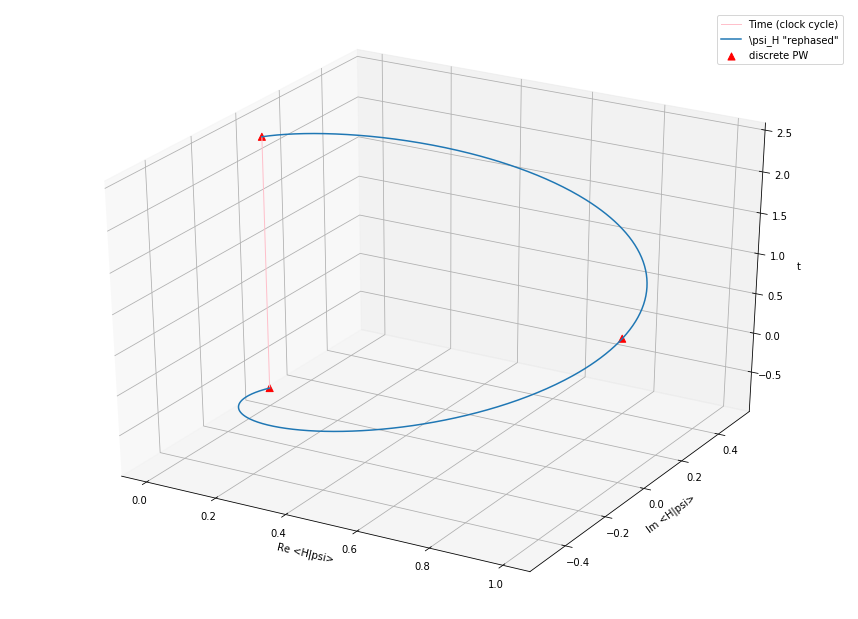
\includegraphics[width=\textwidth]{img/psi_H.png}
  \caption{
    Evolution of $\braket{H}{\psi(t)}$ in the two models.
  }
  \label{fig:psi_H}
\end{figure}

\begin{figure}
  %\centering
  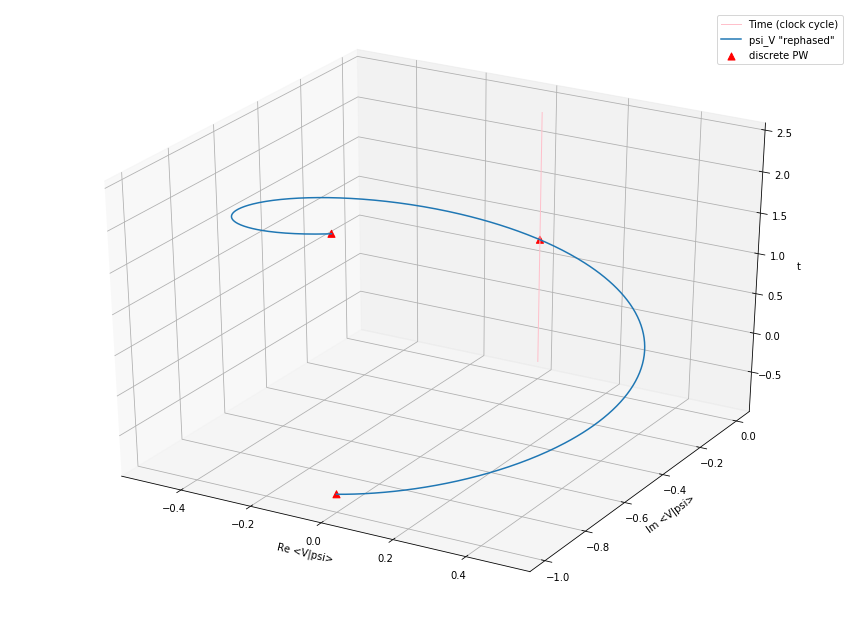
\includegraphics[width=\textwidth]{img/psi_V.png}
  \caption{Evolution of $\braket{V}{\psi(t)}$ in the two models.}
  \label{fig:psi_V}
\end{figure}

\subsection{Increasing the accuracy with a multi-level clock}

\subsubsection{Preliminaries}

A clock that can measure only two times in one cycle of a periodic evolution
is of limited interest ---and limited falsifiability, as it can be easily
interpolated by different models.
The experiment described in
\cite{Moreva:synthetic} and related works attempts at addressing the issue:
\begin{quote}
  To obtain a more interesting clock, we perform the same conditional probability measurement
  introducing varying time delays to the clock photon, implemented through quartz plates of
  variable thickness.
\end{quote}
But it's worth noting that such delay is in fact a classical external parameter.
%
In what follows, instead, our approach to a more interesting clock will be based on simply
increasing the number of levels of the clock, or in other words increasing the
finite dimension of the Hilbert space $\hilb{H}_T$. This is certainly feasible
theoretically, possibly resorting to numerical computation.
\begin{remark}
  Experimentally,
  besides looking for a suitable $N$-level system to act as a clock,
  we may want to ``encode'' $2^{n}$ levels into the combined state of $n$
  qubits and
  decompose $\mathbb{J}$ ---or, actually, $e^{-i\mathbb{J}\tau/\hbar}$---
  into simpler hamiltonians (evolutions)
  acting on individual qubits (\term{gates}),
  therefore allowing the experiment to be run on a quantum computer.\footnote{
    Nevertheless, a quantum computation model based on
    $N$-dimensional \term{qudits}
    (with $N > 2$)
    is considered in the literature \parencite{QuditComp, Qudit}
    as a possible approach to \emph{simplify} implementation
    of more general purpose quantum processors, not only specific experiments.
  }
  A decomposition method that can be considered for the purpose
  is the Trotter-Suzuki scheme
  \parencite{Trotter-Suzuki:exp, Trotter-Suzuki:GPU}.
  This is a potential line of further study.
\end{remark}

\subsubsection{Eigensystem in the product space and consistency with ordinary quantum \mbox{theory}}
\label{sec:building-the-discrete-pw-clock}
Appendix \ref{appendix:n-level} reports the details of
symbolic and
numeric computation for
an $N=32$-level clock, ``timing'' a qubit subject to the same hamiltonian
of the experiment we have seen in eq.~\eqref{eq:H_S}.

In this case, for simplicity, we work in
``natural units'' $\hbar = \omega = 1$, where $\omega$ is
the characteristic frequency in the same sense of the
two-level clock experiment described in \S\ref{1qubitExp}.

The clock is built as having a time operator which is diagonal in the
chosen computational basis\footnote{
  Here there's no explicit reference to any particular physical implementation. 
}:
\[
  \hat{T} \repr \frac{2\pi}{N}
  \begin{pmatrix}
    0           &       &       &       \\
                &1      &       &       \\
                &       &\ddots &       \\
                &       &       &N-1
  \end{pmatrix} \,\text{.}
\]
With this choice, the clock spans the characteristic period of $\Delta T = 2\pi$.

The ``spatial space'' or ``ordinary Hilbert space'' $\hilb{H}_S$
is still 2-dimensional, and the hamiltonian in it is simply
\[
  \hat{H}_S \repr
  i
  \begin{pmatrix}
    0   & 1   \\
    -1  & 0
  \end{pmatrix}
  \, \text{.}
\]

Frequency operator $\hat{\Omega}$ is derived, analytically, via Fourier
transformation as seen in \eqref{eq:SI_Fourier:Omega}:
\[
  \hat{\Omega} = \frac{N}{2\pi} F^{}_{N} \hat{T} F^{\dagger}_{N} \, \text{.}
\]
With a large $N$,
such derivation is extremely laborious. We don't resort to
numeric FFT in this case, but we do benefit of computer-aided, yet exact
symbolic computation.

Once $\hat{\Omega}$ is derived though,
the eigenvalues and eigenvectors of
$\hat{\mathbb{J}} = \hbar\hat{\Omega}\ox\idop_S + \idop_T\ox\hat{H}_S$
can only, realistically, be computed with numerical methods.

In order to illustrate interesting examples, not corresponding to the
trivial evolution of an eigenstate of $H_S$,
but to some kind of Rabi oscillation or Larmor precession
\parencite[Ch. IV]{Cohen-Tannoudji}, we pick, in \term{Mathematica}'s ordering,
eigenvectors $\dket{\Phi_{40}}$ and $\dket{\Phi_{41}}$ of $\hat{\mathbb{J}}$
in $\hilb{H}_T \ox \hilb{H}_T$, corresponding to eigenvalues
$\epsilon_{40} = 12$ and $\epsilon_{41} = 11$.

Each eigenvector encodes a whole possible discrete-time history
of the qubit over a cycle,
as stated in \eqref{eq:timepicks2} or \eqref{eq:timepicksN}.

So, for example, if components $1$ and $2$ of $\dket{\Phi_{41}}$ correspond to
(the components of)
an initial state of the qubit in $\hilb{H}_S$
(i.e at ``ordinary time'' $t=0$); components
$2k + 1$ and $2k + 2$ correspond to $t = \frac{2\pi}{N}k \eqbydef t_k$
of same, $\forall k \in \qty{0, \dots, N-1}$.

A comparison of Page--Wootters results with ordinary
Schr{\"o}dinger evolution is thus given by the comparisons
\begin{align}
  \dbradket{2k+1}{\Phi_{41}} e^{-i \epsilon_{41} t_k} &\sim \braket{0}{\psi(t_k)}_{\mathrm{S}} \label{eq:comparison0} \\
  \dbradket{2k+2}{\Phi_{41}} e^{-i \epsilon_{41} t_k} &\sim \braket{1}{\psi(t_k)}_{\mathrm{S}} \label{eq:comparison1}
  \,\text{,}
\end{align}
where the phase $e^{-i \epsilon_{41} t_k}$ is motivated in \cite[``The Zero-eigenvalue'']{Lloyd:Time},
and inessential if one is merely interested in determining and comparing probabilities
$\qty|\braket{0,1}{\psi}|^2$. Please note the double angle bracket notation for vectors
and algebraic operations in the product space $\hilb{H}_T \ox \hilb{H}_S$.

\begin{figure}
  \centering
  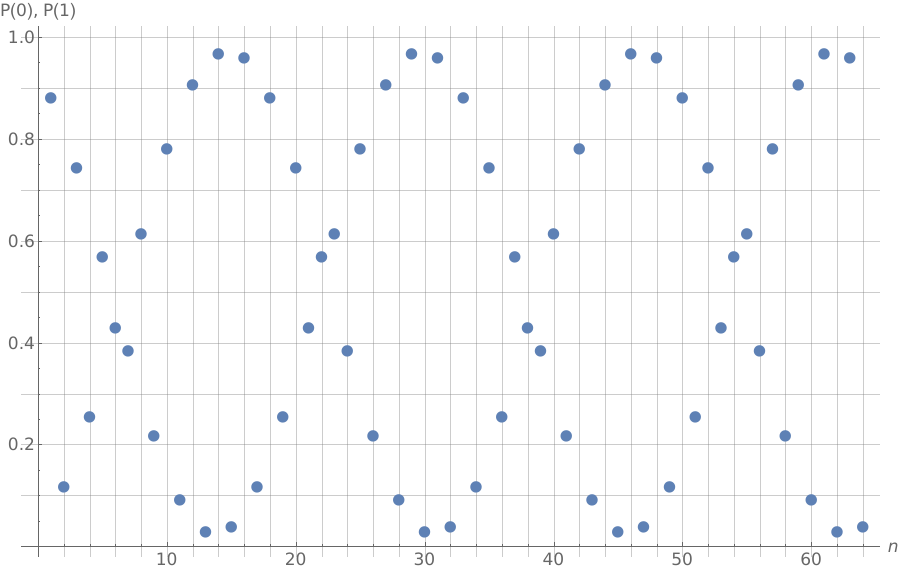
\includegraphics[height=.3\textheight]{img/N32-B.png}
  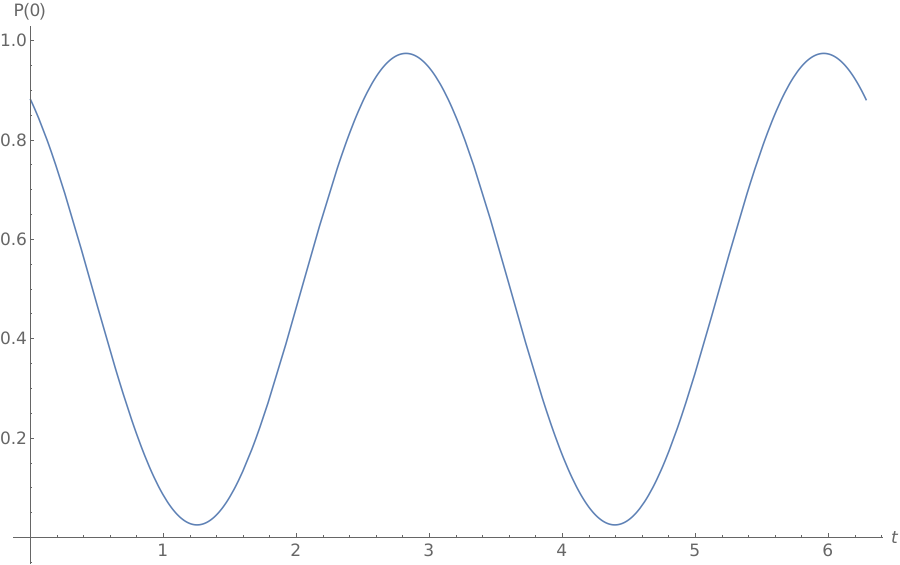
\includegraphics[height=.3\textheight]{img/probB_0.png}
  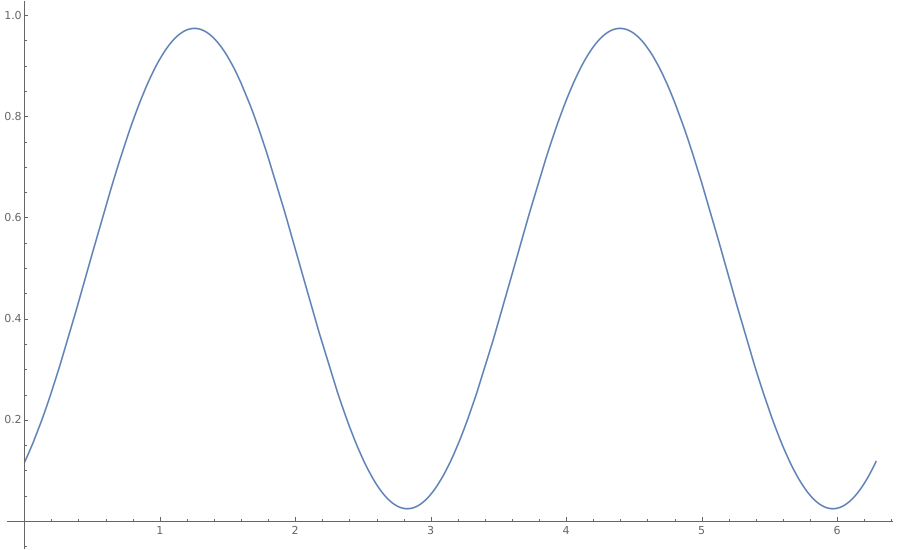
\includegraphics[height=.3\textheight]{img/probB_1.png}
  \caption{P-W vs Schr{\"o}dinger probability evolution for $\hat{\mathbb{J}}$ eigenvalue $=11$}
  \label{fig:prob-comparison}
\end{figure}

Figure \ref{fig:prob-comparison} is the graphical representation of (the square modulus of)
\eqref{eq:comparison0} and \eqref{eq:comparison1} i.e. the probability for the qubit
in $\hilb{H}_S$ to be $\ket{0}$ or $\ket{1}$.

The discrete graph, on top, plots the
square modulus of components of $\hat{\mathbb{J}}$'s eigenvector $\dket{\Psi_{41}}$.

Odd-index ($2k+1$) square-modulus components
---occupying vertical \emph{spaces} on the grid---
are compared
with the Schr{\"o}dinger evolution of probability $\qty|\braket{0}{\psi}|^{2}$
(first continuos plot, middle image).

Even-index ($2k+2$) components
---occupying vertical \emph{lines} on the grid---
are analogously compared
with the Schr{\"o}dinger evolution of probability $\qty|\braket{1}{\psi}|^{2}$
(second continuos plot, bottom image).

\begin{figure}
  \centering
  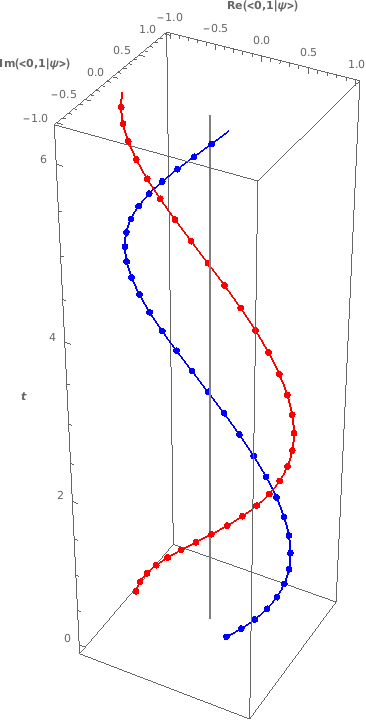
\includegraphics[width=0.45\textwidth]{img/PWfit32.png}
  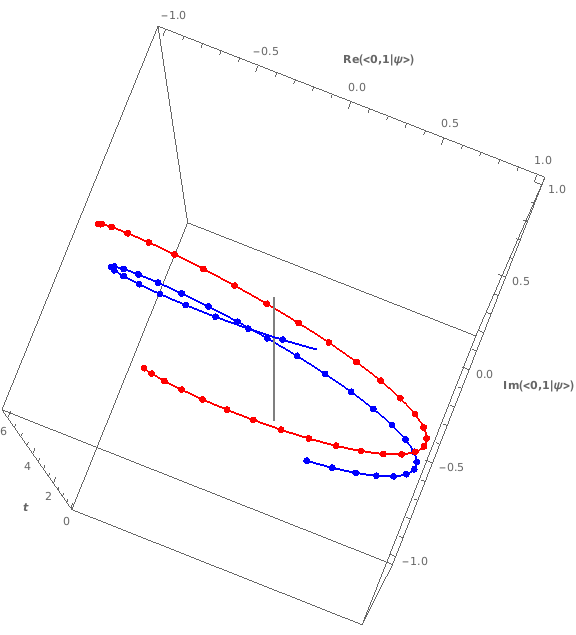
\includegraphics[width=0.5\textwidth]{img/PWfit32top.png}
  \caption[
    P-W vs Schr{\"o}dinger evolution (complex values)
  ]{
    Page--Wootters discrete-time ``evolution without evolution'' (points)
    is interpolated by the (continuous lines) of standard quantum mechanics
    evolution.
    Horizontal axis are real and imaginary part of the wave function components.
    Vertical axis is time $t$.
    Red   line plots {\color{red}   $\braket{0}{\psi(t)}$}.
    Blue  line plots {\color{blue}  $\braket{1}{\psi(t)}$}.
  }
  \label{fig:complex-comparison}
\end{figure}

Finally, Figure \ref{fig:complex-comparison} compares the two sides of
\eqref{eq:comparison0} and \eqref{eq:comparison1}
in terms of \emph{complex value}
(%
  therefore the term $e^{-i \epsilon t_k}$ is relevant,
  for eigenvalues $\epsilon \neq 0$ of $\hat{\mathbb{J}}$%
).
